\part{从蓝光二极管到OLED的现代化进程}

\section{从蓝光LED到白光LED}
\begin{slide}
\begin{enumerate}[1.]
    \item 1961年美国公司德州仪器的Robert Biard与Gary Pittman首次发现了砷化镓及其他半导体合金的红外放射作用,也就是红光LED,标志着LED的诞生
    \item 过了30多年, 到1993年蓝光LED的发明, 才标志着LED的全彩时代拉开帷幕
    \item 蓝光二极管的重要性不仅在于它本身,更在于推动了白光二极管的诞生,也就是目前广泛用于生产生活的灯源
\end{enumerate}
\end{slide}

\section{白光LED的制造}

\begin{slide}
有了能发出蓝光的发光二极管就可以制造白光LED，主要有以下两种制造方式:
\begin{enumerate}[1]
    \item 这种方法涉及用不同颜色的荧光粉涂覆一种颜色的LED（主要是由InGaN制成的蓝色LED）以形成白光；由此产生的LED称为基于荧光粉或荧光粉转换的白光LED（pcLED）。一小部分蓝光经历Stokes位移，将其从较短的波长转变为更长的波长。使用几个不同颜色的荧光粉层可以扩大发射光谱，有效地提高显色指数（CRI）。\\
    \textit{优点：制造简单，亮度高}\\
    \textit{缺点：LED发出的光能有一部分被转化成热能，效率较低}
    
    \item 结合蓝光发光二极管、红光发光二极管和绿光发光二极管便可做出白光发光二极管\\
    \textit{优点:有较广的色域,并且发光效率较高}\\
    \textit{缺点:具有较高的制作成本}
\end{enumerate}
\end{slide}

\begin{slide}{荧光粉基发光二极管}
    第一种白光LED采用了掺杂铈的钇铝石榴石（Ce:YAG），这是一种荧光粉，在受到蓝色光照射时会发出黄光（Stokes偏移）。作为高亮度蓝色InGaN二极管上的涂层，将部分蓝光转换为黄色，然后一起显示为白色。
    \begin{figure}
        \centering
        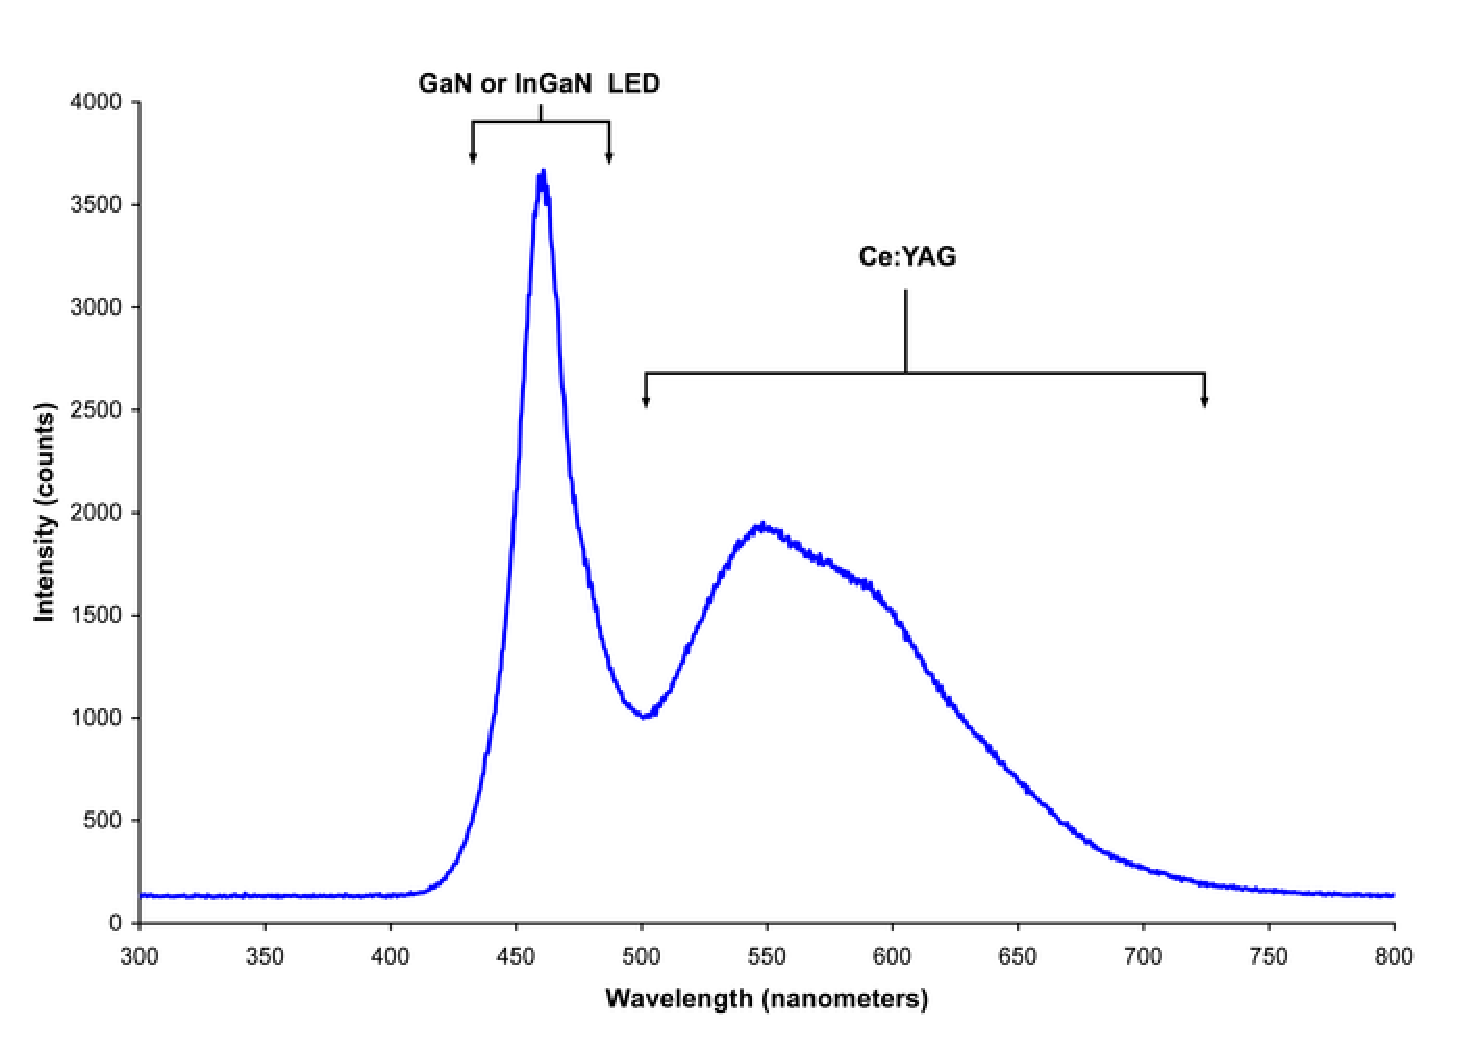
\includegraphics[width=0.5\linewidth]{sep3_images/700px-White_LED.pdf}
        \caption{白光LED的光谱显示基于GaN的LED直接发射的蓝光（峰值约为465 nm）和Ce:YAG荧光粉发出的更宽带的Stokes偏移光，其发射波长约为500 -- 700 nm}
    \end{figure}
\end{slide}

\begin{slide}{荧光粉基发光二极管}
    基于荧光粉的LED由于Stokes位移和其他与磷光体相关的问题导致的热损失而产生效率损失。与普通LED相比，它们的发光效率取决于所产生光输出的光谱分布和LED的原始波长。截至2010年，最有效的黄色荧光粉仍然是YAG荧光粉，Stokes位移损耗不到10\%。
    \\~\\
    由于制造简单，荧光粉法仍然是制造高强度白光LED的最常用方法。使用具有荧光粉转换的单色发射器设计和生产光源比复杂的RGB系统更简单，更便宜，目前市场上的大多数高强度白光LED都是使用荧光粉光转换制造的。
\end{slide}

\begin{slide}{荧光粉基发光二极管}
    还有一种荧光粉基发光二极管类似于日光灯，发光单元是近紫外发光二极管，外面包着两种磷光剂混合物，一种是发红光和蓝光的铕，另一种磷光剂是发绿光的铜和铝掺杂了硫化锌。内里的紫外光发光二极管发出的紫外光被外层的磷光剂转换成红、蓝、绿三色光，混合后就成了白光。
    \\~\\
    \textit{优点:光谱的特性较佳，产生的光比较好看}\\
    \textit{缺点:紫外线会使黏合剂中的环氧树脂劣化变质，所以生产难度较高，而寿命亦较短,光波在转化过程中有较多被化成热能，因此效率较低}
\end{slide}

\begin{slide}{RGB系统}
    混合红色、绿色和蓝色光源以产生白光需要电子电路来控制颜色的混合。由于不同颜色发光模式略有不同，即使RGB光源封装在单个LED中，色彩平衡也可能根据视角而改变，因此RGB二极管很少用于产生白光。尽管如此，由于混合不同颜色的灵活性，这种方法有许多应用，原则上，这种机制在产生白光方面也具有更高的量子效率。
    \\~\\
    有几种类型的多色白光LED：二色、三色和四色白光LED。在这些不同方法中起作用的几个关键因素包括颜色稳定性，显色能力和发光效率。通常，更高的效率意味着更低的显色性，从而在发光效率和显色性之间进行了权衡。其中一个挑战是开发更高效的绿色LED，它的理论最大值为683 lm/W，但很少有绿色LED超过每瓦100流明，蓝色和红色LED接近其理论极限。
\end{slide}

\begin{slide}{RGB系统}
    \begin{columns}
        \begin{column}{0.5\linewidth}
            \begin{figure}
            \centering
            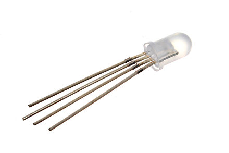
\includegraphics[width=0.8\linewidth]{sep3_images/440px-RGB_LED.pdf}
            \caption{封装在一起的红色和绿色LED}
            \end{figure}
        \end{column}
        \begin{column}{0.5\linewidth}
            \begin{figure}
            \centering
            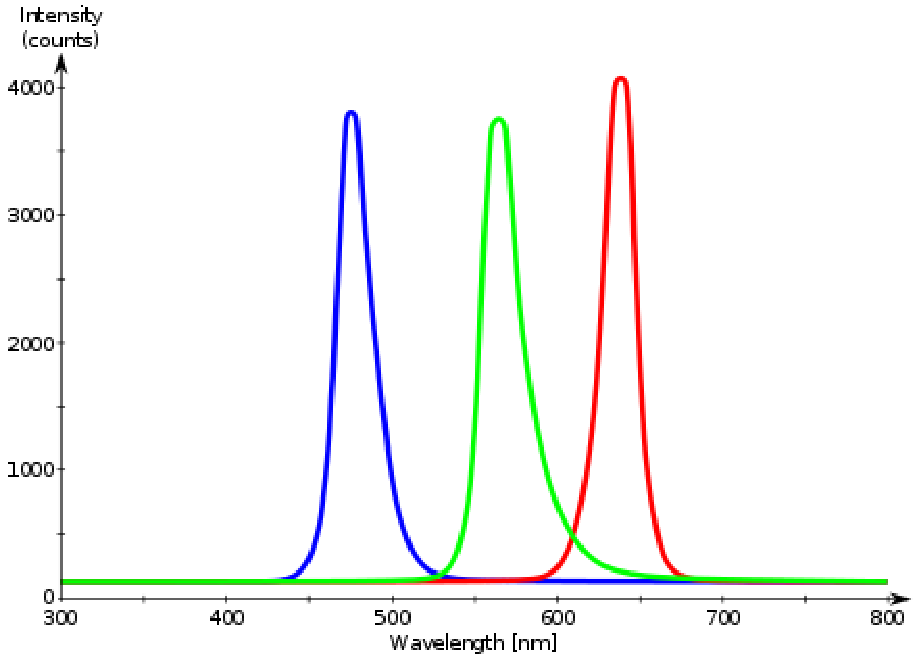
\includegraphics[width=0.8\linewidth]{sep3_images/440px-RGB_LED_Spectrum.pdf}
            \caption{蓝色、黄绿色和高亮度红色固态半导体 LED 的组合光谱曲线。光谱带宽约为24 -- 27 nm}
            \end{figure}
        \end{column}
    \end{columns}
\end{slide}

\begin{slide}{RGB系统}
    多色LED还提供了一种形成不同颜色的光的新方法。大多数可感知的颜色可以通过混合不同量的三原色来形成。这允许精确的动态色彩控制。然而，这种类型的LED的发射功率随着温度的升高而呈指数级衰减，导致颜色稳定性发生巨大变化，这抑制了它的工业用途。
    \\~\\
    没有荧光粉的多色LED无法提供良好的显色性，因为每个LED都是窄带光源。没有荧光粉的LED虽然是一种较差的普通照明解决方案，但对于基于LED直接像素的显示器来说，这是最佳解决方案。
\end{slide}

\section{发光二极管(LED)的应用}
\begin{slide}
\textbf{状态显示灯:}
\begin{enumerate}[]
    \item
    \textit{发光二极管所需推动电压及功率低，方便由运作电压低的微处理器控制及在以电池作电源的设备上使用，所以常被用在各种电子产品、设备的状态指示灯。在消费性电子产品，手提嵌入式电子设备，家庭电器、玩具、各种仪器……等用途上作为工作状态显示灯。}
    \begin{figure}[H]
        \centering
        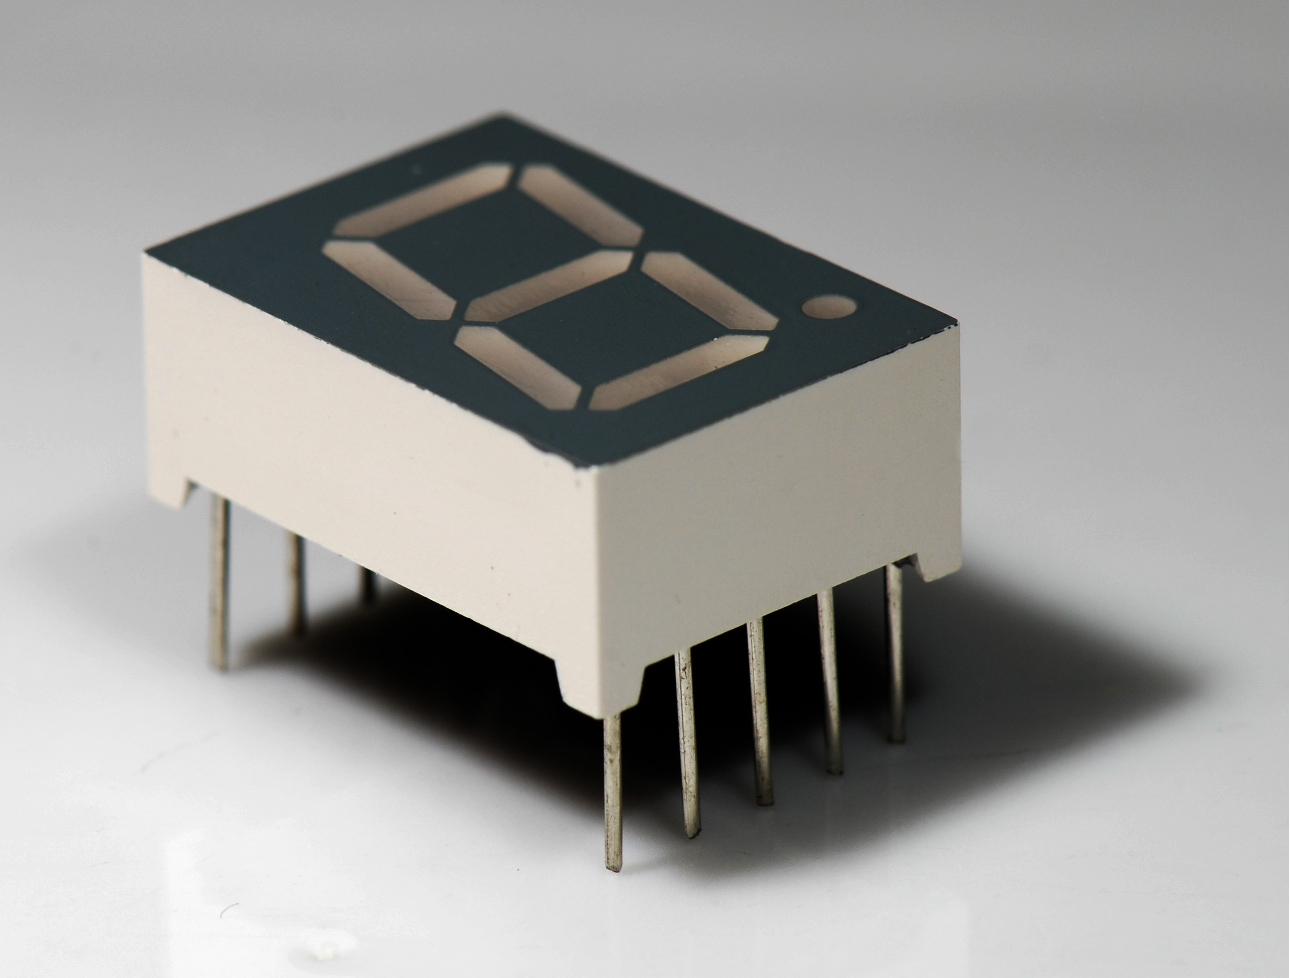
\includegraphics[height=4cm, width=6cm]{sep3_images/Seven_segment_02_Pengo.pdf}
        \caption{用来制作数字显示器的发光二极管元件}
    \end{figure}
\end{enumerate}
\end{slide}

\begin{slide}
\textbf{交通道路指示灯}
\begin{enumerate}[1.]
    \item 在车辆上的应用：\\
    \textit{当LED的光度发展达至要求后，便有汽车用LED作转向与刹车灯，主要好处是LED极高的开关速度，其亮起时间比白炽灯快$\mathrm{0.5s}$之多，且LED灯在白天时与白炽灯炮相比亮度较高、使用寿命长、点亮速度快，更可增加$\mathrm{6m}$的刹车辨识距离，也可降低事故发生，这对行车安全非常重要。而车辆行驶环境中震荡、温差变化下，LED仍然有稳定的光度及可靠性。}
    \item 在道路上的应用：\\
    \textit{同样工作在户外环境的交通灯使用开关快速的LED也很适合，LED寿命较长也减少坏灯及影响交通的机会。}
    \item 公共场所的平板显示器：\\
    \textit{在机场、机舱、火车站、巴士站、码头等…各种公共交通工具上等地方，LED被普遍地采用作为平板显示器以显示如班次、目的地、时间等相关讯息。而LED的可靠性与低耗电，使其也适合用作紧急出口指示灯。}
\end{enumerate}
\end{slide}

\begin{slide}
\textbf{LED照明:}\\
由于发光二极管灯被称为固态照明。传统照明灯俱如萤光灯、白炽灯及卤素灯都有装载气体的脆弱玻璃管，因而都不及全固态的LED坚固耐用。由于发光二极管在增加光度时，效率会下降，所以有些LED灯使用多个白光LED组合成一簇构成一个光源，以增加效率；同样的原因，在照明方面只用在对光度要求低的地方，以保持其较佳效率（省电）的特性，这些用途包括：
\begin{enumerate} [1.]
    \item 手电筒
    \item 紧急照明
    \item 手机闪光灯
    \item 道路及室内照明
\end{enumerate}
\end{slide}

\begin{slide}
\textbf{LCD显示器背光光源:}
\begin{enumerate}[]
    \item
    \textit{早在只有黑白LCD的年代（当时并未有蓝色及白色LED），各种单色LED便被采用作黑白LCD的背光光源，例如传呼机，而当彩色LCD出现后多时，工程界还未能制作出白色LED，所以只好采用电致发光片，简称EL片,作背光。而在白色LED出现后，这些产品随即转用LED作背光。与EL片相比，白色LED较省电，这对电池供电的产品特别重要，除此之外，白色LED免去EL片所需的高压电源，大大减低了电磁干扰。但由于白色LED需要一定空间作导光之用，体积会比EL片略厚，尽管如此，手提电话、电子手帐、较细的手提电脑续渐使用LED作背光。}
\end{enumerate}
\end{slide}

\begin{slide}
\textbf{显示器:}
\begin{enumerate}
    \item \textit{市面上现存普及的LED背光液晶显示电视的LED只用作背光光源，严格上并不是LED显示器，细小高解像度的视讯LED显示器现都采用OLED，OLED具有自发光性、广视角、高对比、低耗电、高反应速率等优点，OLED显示器因为不需背光源，所以可以比LCD显示器造得更薄}
    \item \textit{大型的LED显示器已普及于户外户内，户外LED显示器对解析度要求较低，但需要较高的亮度，多采用分立单色的LED组成。}
\end{enumerate}
\end{slide}

\section{有机发光二极管(OLED)}
\begin{slide}
有机发光二极体OLED。其发光原理跟发光二极管一样，不同之处是其发光物半导体是有机化合物（有机半导体），例如有机聚合物等。OLED制造流程简单，成本较低，可以用印刷等廉价生产方法制造，其优点包括：
\begin{enumerate}
    \item \textit{可以制造出大面积的面光源}
    \item \textit{元件本身可以是柔软、透明的}
\end{enumerate}
这些特性都是一般二极管所不及的。因此OLED可以造出大面积的照明灯具，软身、透明的显示器。
\end{slide}

\begin{slide}
有机发光二极体基本结构是由一薄而透明具半导体特性之铟锡氧化物（ITO），与电力之正极相连，再加上另一个金属阴极，包成如三明治的结构。整个结构层中包括了：电洞传输层（HTL）、发光层（EL）与电子传输层（ETL）。当电力供应至适当电压时，阳极空穴与阴极电子便会在发光层中结合，产生光子，依其材料特性不同，产生红、绿、蓝三原色，构成基本色彩。
    \begin{figure}[H]
        \centering
        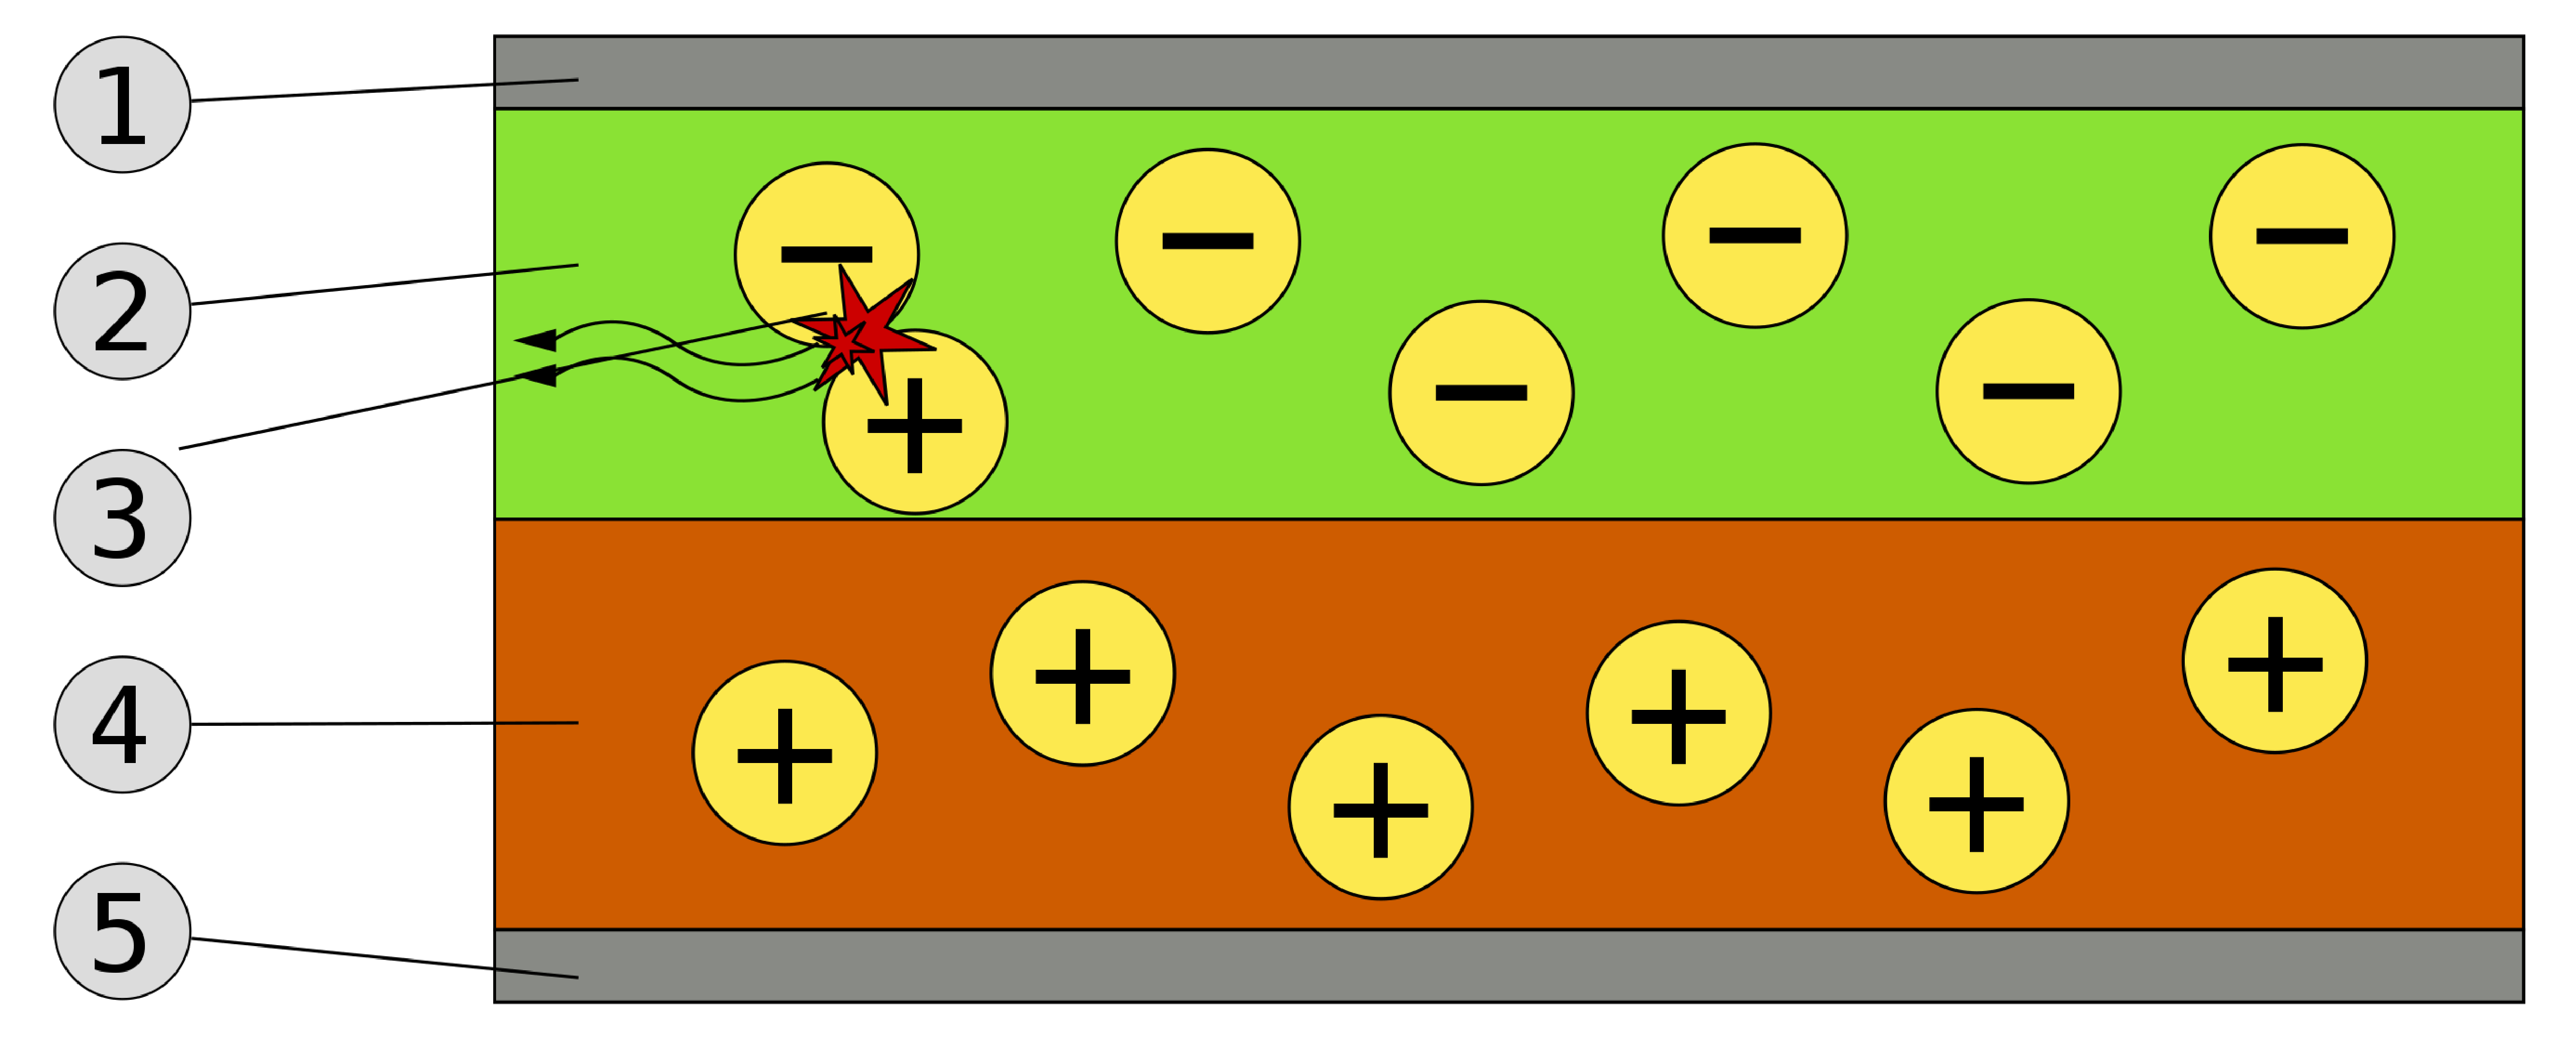
\includegraphics[height=2cm, width=6cm]{sep3_images/OLED_schematic.pdf}
        \caption{OLED基本结构：1. 阴极 (−)；2. 发光层（Emissive Layer, EL）；3. 阳极空穴与阴极电子在发光层中结合，产生光子；4. 导电层（Conductive Layer）；5. 阳极 (+)}
    \end{figure}
\end{slide}

\begin{slide}
最早的OLED技术研发开始于1950年代的法国南茜大学，法国物化学家安德烈·贝纳诺斯获誉为“OLED之父”，最早的实用性OLED于1987被柯达公司的中国香港人邓青云和美国人史蒂夫·范·斯莱克两人发现.
\begin{enumerate}[]
    \item \textit{邓青云自1975年开始加入柯达公司Rochester实验室从事有机发光二极体的研究工作，在意外中发现有机发光二极体。1979年的一天晚上，他在回家的路上忽然想起有东西忘记在实验室，回到实验室后，他发现在黑暗中的一块做实验用的有机蓄电池在闪闪发光，从而开始了对有机发光二极体的研究。1987年，邓青云和同事史蒂夫·范·斯莱克成功地使用类似半导体 PN结的双层有机结构第一次作出了低电压、高效率的光发射器。为柯达公司生产有机发光二极体显示器奠定了基础。}
\end{enumerate}

OLED英文名为Organic Light-Emitting Diode，缩写：OLED，中文名“有机发光二极管”都是邓青云命名的。
\end{slide}

\begin{slide}
OLED的特性是自发光，不像薄膜电晶体液晶显示器需要背光，因此可视度和亮度均高，且无视角问题，其次是驱动电压低且省电效率高，再加上反应快、重量轻、厚度薄，构造简单，成本低等特点，被视为21世纪最具前途的产品之一。
\\~\\
OLED可应用于制造平价可弯曲显示器、照明设备、发光衣或装饰墙壁。2004年开始，有机发光二极体已广泛应用于随身MP3播放器。不同颜色的OLED有不同寿命，衰退程度也不同（蓝色OLED的寿命最短），因此作为全彩色显视器时，色温会随使用时间而变，较常用的像点会较其他像点衰退得较快而使得光暗不均和偏色，也就是OLED显示器的“烧屏”（screen burn-in）现象。水份、湿气等会对OLED造成破坏，因此对封装的防水性也有要求。
\end{slide}

\begin{slide}
从技术上讲，问题在于蓝色LED的发光效率明显低于红色或绿色像素。这意味着，蓝色LED需要以更高的电流驱动，才能达到与红色或绿色像素相同的亮度。更高的电流会导致像素更快地退化，缩短其寿命，从而最终使显示屏的颜色向红色和绿色倾斜。因此OLED显示屏的颜色并不是均匀退化的，它最终会以红/绿色调呈现。因此，如果面板的某一区域长期显示蓝色或白色的图像，那么这个区域的蓝色像素会比其他区域退化得更快。这是烧屏产生的根本原因。
\\~\\
一般来讲，蓝色的OLED寿命最短，绿色OLED的寿命最长，因此厂家通过使蓝色、红色子像素变大，这样就需要更少的电流来驱动以提供所需的光，以增加它们的寿命，需要更长的时间才会出现明显的色彩变化。这就出现了Pentile排列和Diamond Pentile排列。
\end{slide}

\begin{slide}
    \begin{columns}
        \begin{column}{0.5\linewidth}
            \begin{figure}
            \centering
            
\includegraphics[width=\linewidth]{sep3_images/Screen_Burn-in.pdf}
            \caption{由于长时间显示新闻栏目产生的烧屏现象}
            \end{figure}
        \end{column}
        \begin{column}{0.5\linewidth}
            \begin{figure}
            \centering
            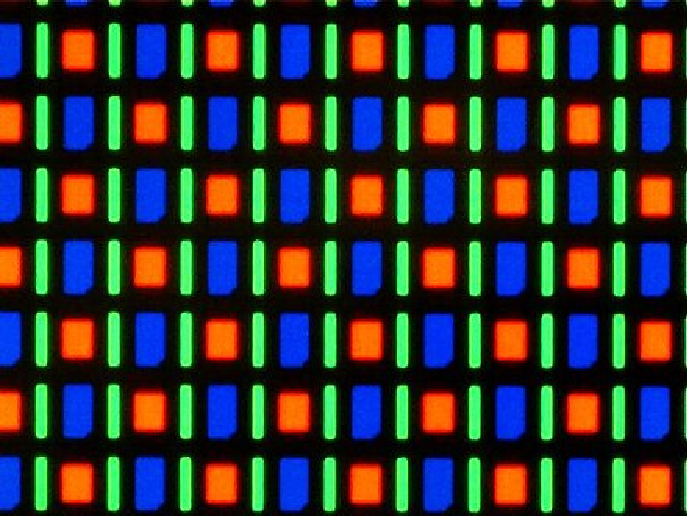
\includegraphics[width=.8\linewidth]{sep3_images/Pentile.pdf}
            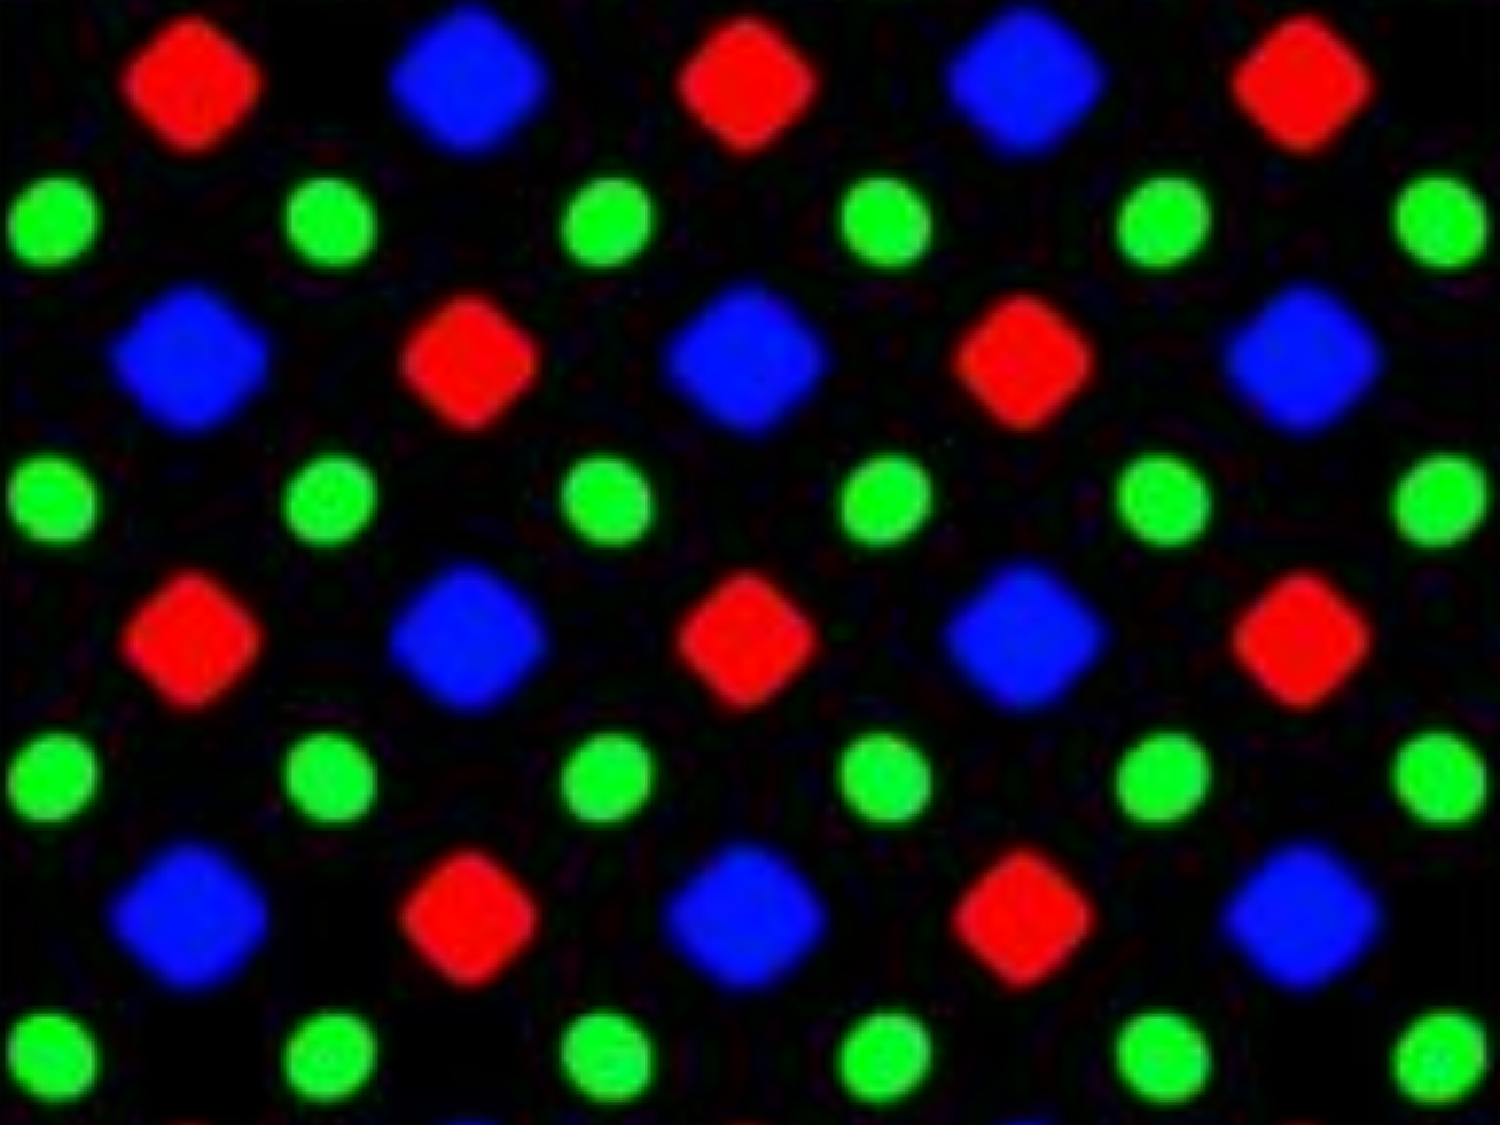
\includegraphics[width=.8\linewidth]{sep3_images/Diamond_Pentile.pdf}
            \caption{Pentile排列（上）和Diamond Pentile排列（下）}
            \end{figure}
        \end{column}
    \end{columns}
\end{slide}

\begin{slide}
此外，OLED还在光医学领域有广泛前景:
\begin{enumerate}
    \item 治疗创伤（PBM光疗法）：相比传统光医疗，OLED 贴片凭借二维弯曲（柔性）、轻薄、可穿戴等特点，可以更贴合皮肤，舒适感和体验性会更佳。
    \item 可穿戴OLED发光器件在个人移动医疗监测领域来测量人体信号，例如监测心跳和血氧水平。这是因为在心血管监测方法中，光体积描记法（PPG）信号和血氧饱和度（SpO2）水平是通过使用发光器件和光检测器，进行无创光测量的。
\end{enumerate}
\end{slide}
